%%%%%%%%%%%%%%%%%%%%%%%%%%%%%%%%%%%%%%%%%
% baposter Landscape Poster
% LaTeX Template
% Version 1.0 (11/06/13)
%
% baposter Class Created by:
% Brian Amberg (baposter@brian-amberg.de)
%
% This template has been downloaded from:
% http://www.LaTeXTemplates.com
%
% License:
% CC BY-NC-SA 3.0 (http://creativecommons.org/licenses/by-nc-sa/3.0/)
%
%%%%%%%%%%%%%%%%%%%%%%%%%%%%%%%%%%%%%%%%%

%----------------------------------------------------------------------------------------
%	PACKAGES AND OTHER DOCUMENT CONFIGURATIONS
%----------------------------------------------------------------------------------------

\documentclass[landscape,a1paper,fontscale=0.47]{baposter} % Adjust the font scale/size here

\usepackage{graphicx} % Required for including images
\graphicspath{{figures/}} % Directory in which figures are stored

\usepackage{amsmath} % For typesetting math
\usepackage{amssymb} % Adds new symbols to be used in math mode

\usepackage{booktabs} % Top and bottom rules for tables
\usepackage{enumitem} % Used to reduce itemize/enumerate spacing
\usepackage{palatino} % Use the Palatino font
\usepackage[font=small,labelfont=bf]{caption} % Required for specifying captions to tables and figures

\usepackage{multicol} % Required for multiple columns
\setlength{\columnsep}{1.5em} % Slightly increase the space between columns
\setlength{\columnseprule}{0mm} % No horizontal rule between columns

\usepackage{tikz} % Required for flow chart
\usetikzlibrary{shapes,arrows} % Tikz libraries required for the flow chart in the template

\newcommand{\compresslist}{ % Define a command to reduce spacing within itemize/enumerate environments, this is used right after \begin{itemize} or \begin{enumerate}
\setlength{\itemsep}{1pt}
\setlength{\parskip}{0pt}
\setlength{\parsep}{0pt}
}

\definecolor{lightblue}{rgb}{0.27,0.62,1} % Defines the color used for content box headers
\definecolor{darkgrey}{rgb}{0.27,0.27,0.27} % Defines the color used for content box headers

\begin{document}

\begin{poster}
{
headerborder=closed, % Adds a border around the header of content boxes
colspacing=1em, % Column spacing
bgColorOne=white, % Background color for the gradient on the left side of the poster
bgColorTwo=white, % Background color for the gradient on the right side of the poster
borderColor=lightblue, % Border color
headerColorOne=darkgrey, % Background color for the header in the content boxes (left side)
headerColorTwo=lightblue, % Background color for the header in the content boxes (right side)
headerFontColor=white, % Text color for the header text in the content boxes
boxColorOne=white, % Background color of the content boxes
textborder=roundedright, % Format of the border around content boxes, can be: none, bars, coils, triangles, rectangle, rounded, roundedsmall, roundedright or faded
eyecatcher=true, % Set to false for ignoring the left logo in the title and move the title left
headerheight=0.1\textheight, % Height of the header
headershape=roundedright, % Specify the rounded corner in the content box headers, can be: rectangle, small-rounded, roundedright, roundedleft or rounded
headerfont=\Large\bf\textsc, % Large, bold and sans serif font in the headers of content boxes
%textfont={\setlength{\parindent}{1.5em}}, % Uncomment for paragraph indentation
linewidth=1.5pt % Width of the border lines around content boxes
}
%----------------------------------------------------------------------------------------
%	TITLE SECTION 
%----------------------------------------------------------------------------------------
%
{
\includegraphics[height = 6em]{wits-logo-1.jpg}} % First university/lab logo on the left
{\bf\textsc{ParkSmart - An IoT Parking System for a Smart Campus }\vspace{0.5em}} % Poster title
{\textsc{ Jared Ping \& Lara Timm  \hspace{5pt} \normalsize{School of Electrical \& Information Engineering, University of the Witwatersrand}}} % Author names and institution 
{
\includegraphics[height=7em]{eie-logo.pdf}} % Second university/lab logo on the right


\headerbox{Introduction}{name=introduction,column=0,row=0}{
	The Internet of Things (IoT) is the interconnection of everyday objects, via embedded computing devices and the internet, for the purpose of sending and receiving data. 	\vspace{2mm}

	An IoT-based smart parking system enables the availability of parking spaces to be communicated to a user via a user-friendly mobile application. By directing drivers to available parking spaces, the frustration of finding a place to park is mitigated; saving both time and money.
	\vspace{1mm}
}

\headerbox{Objectives}{name=objectives,column=0,row=1,below=introduction}{
	\begin{itemize}[leftmargin=13pt]\compresslist
		\item Develop a system which can accurately and reliably communicate parking availability in real time
		\item Provide the most feasible cost effective solution
		\item Keep the system energy efficient, maximising \\operational time on a single battery charge
		\item Make the system scalable to accommodate any parking lot size
		\item Ensure the system is robust and easy to maintain
		\item Communicate data through a user-friendly mobile\\ application, built using the Android framework
	\end{itemize}
}

\headerbox{System Design}{name=sysdesign1,column=0,below=objectives,bottomaligned=bottom}{ 
	\begin{center}
		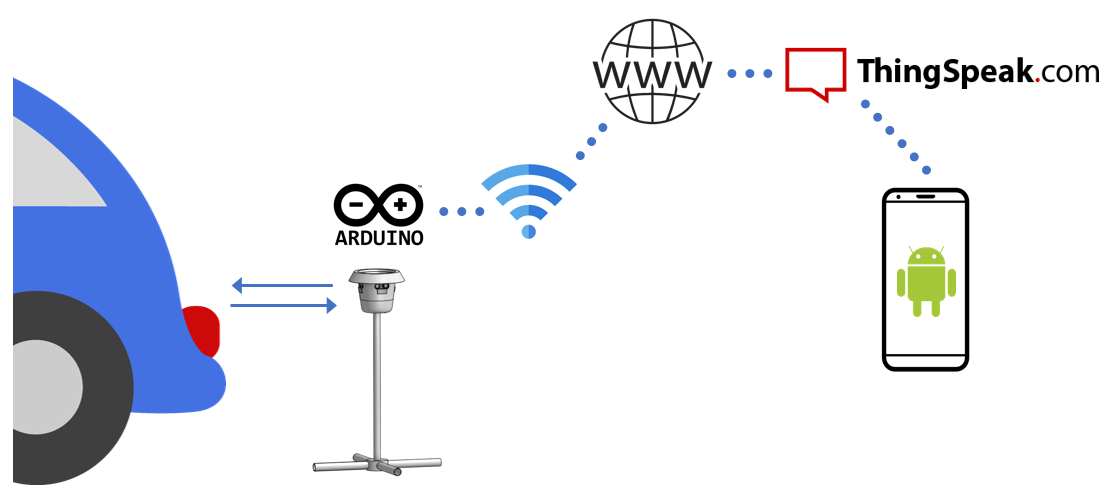
\includegraphics[width=0.9\columnwidth]{Picture2}
		\captionof{figure}{A high-level depiction of the implemented system}
		\raggedright
	\end{center}
\vspace{-1mm}

	\textbf{System Features}
		\begin{itemize}[leftmargin=13pt]\compresslist
			\item The availability of 72 parking spaces is monitored
			\item Empty spaces are communicated to users through a user-friendly mobile application
			\item Parking availability status is updated every 30~seconds
			\item Operates during active parking hours (7~am - 3~pm)
			\item Fail-safes are in place to mitigate node failures
		\end{itemize}
	
	\textbf{Hardware Setup}
		\begin{itemize}[leftmargin=13pt]\compresslist
			\item Ultrasonic distance measurement sensor
			\item Arduino Nano microprocessor
			\item 2.4~GHz radio module
			\item 2*AA rechargeable 2300~mAh NiMh batteries
			\item 5~V boost converter
			\item ESP8266 based Wi-Fi module
		\end{itemize}

}

\headerbox{System Design (cont.)}
{name=sysdesign2,column=1,span=2,row=0}{ 
	\begin{multicols}{2}
		
		\textbf{Software Setup}
			\begin{itemize}[leftmargin=13pt]\compresslist
				\item A scalable Wireless Sensor Network (WSN) utilising 2.4GHz RF communication is designed
				%\item  A scalable RF communication mesh network is designed 
				\item To maintain a low cost node design, system complexity increases with increasing number of parkings
				\item Sensor data is aggregated and uploaded according to the node hierarchy depicted in Figure~2
				\begin{center}
					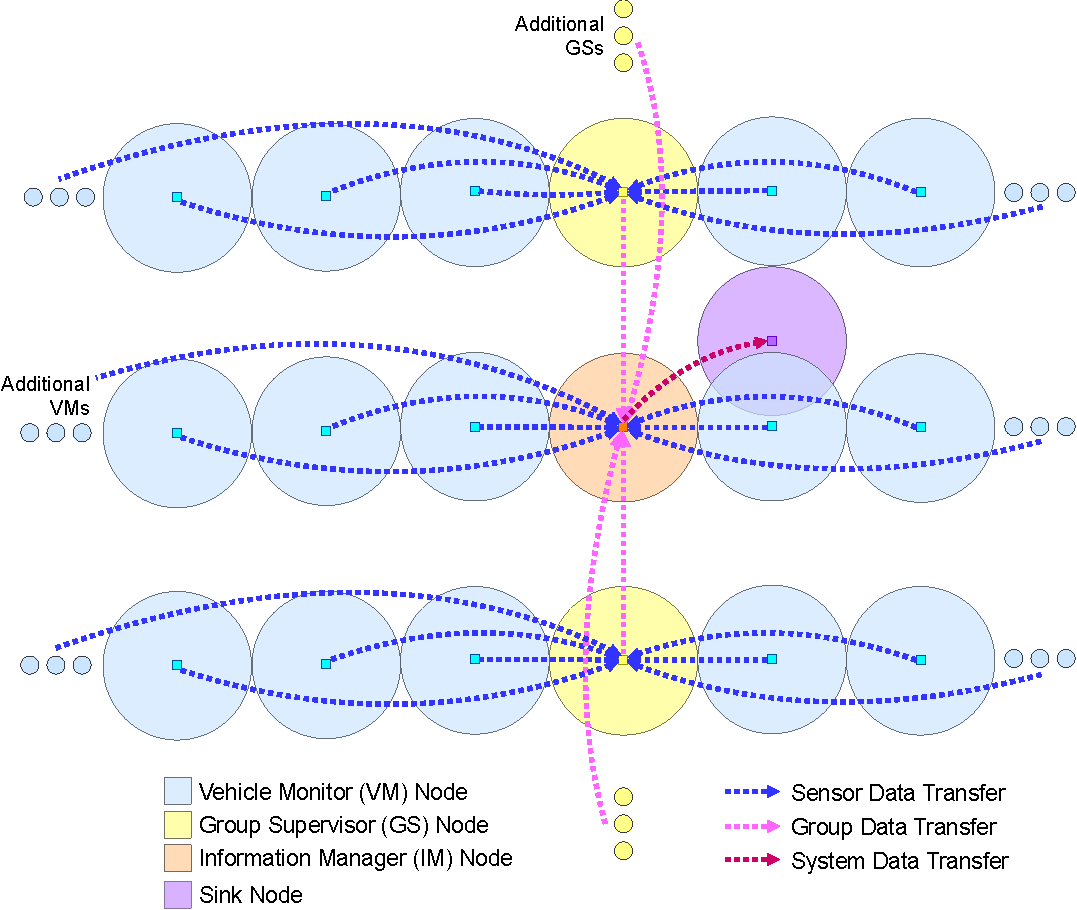
\includegraphics[width=0.84\columnwidth]{mesh-cropped}
					\captionof{figure}{Visulisation of the flow of data, during retrieval, from Sensor Nodes to Sink Node}
				\end{center}
			\vspace{0.5mm}
				\item Data upload is optimised by utilising the ThingSpeak MQTT broker
					\begin{itemize}[leftmargin=13pt]\compresslist
						\item Speedy connection and upload time
						\item Small payload size
					\end{itemize}
				\item An intuitive mobile application is built for Android
				\item Parking lot data is retrieved by the application through the provided ThingSpeak API
				%\item Mobile application automatically refreshes with updated parking bay availability data
				\item The application automatically updates, ensuring up-to-date parking lot data is always displayed 
			\end{itemize}
		
		
	
		\textbf{Smart System Operation}
			\begin{itemize}[leftmargin=13pt]\compresslist
				\item A full cycle (see Figure~3) incurs an average operation time of approximately 1.6~seconds
				\item The mobile application highlights non-transmitting nodes, indicating system fault to network managers
			\end{itemize}
		
		\vspace{1mm}
		
		\begin{center}
			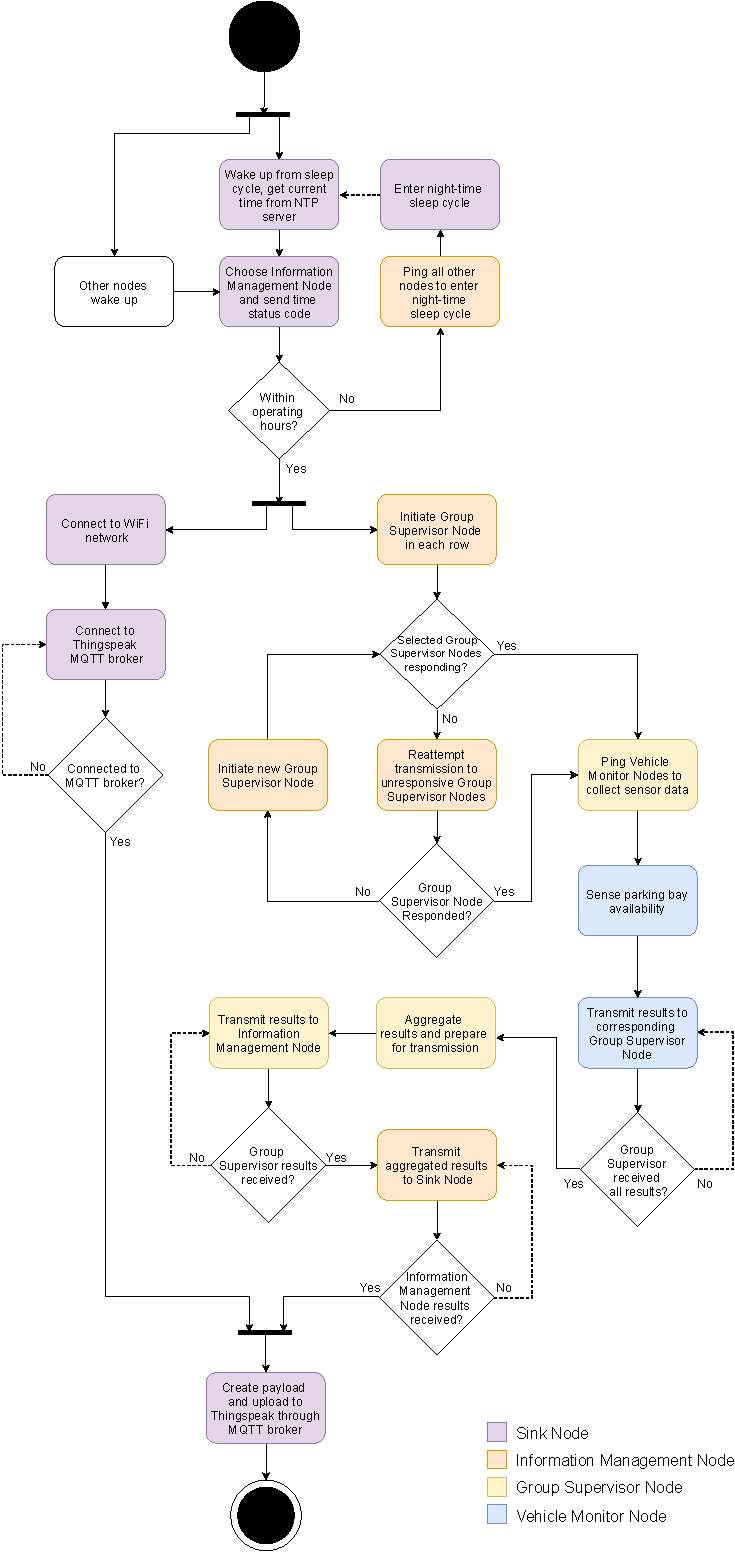
\includegraphics[width=0.9\columnwidth]{flowFinalPoster-cropped}
			\captionof{figure}{Detailed system interactions between role specific nodes per cycle during operational hours}
		\end{center}
	
	\end{multicols}
}

\headerbox{Deployment}{name=deployment,column=1,row=1,span=2, below=sysdesign2,bottomaligned=bottom}{
	\begin{multicols}{2}
		
		\textbf{Construction Specifics} 
		\begin{itemize}[leftmargin=13pt]\compresslist
			\item PCB design for optimized system production
			\item 3D printed sensor holders allow customised sensor placement within each node
			\item Waterproof encasing and tamper-proof lid
			\item Robust stand, prevents damage caused by rain runoff
		\end{itemize}
	
	\vspace{1em}
	
		\begin{center}
			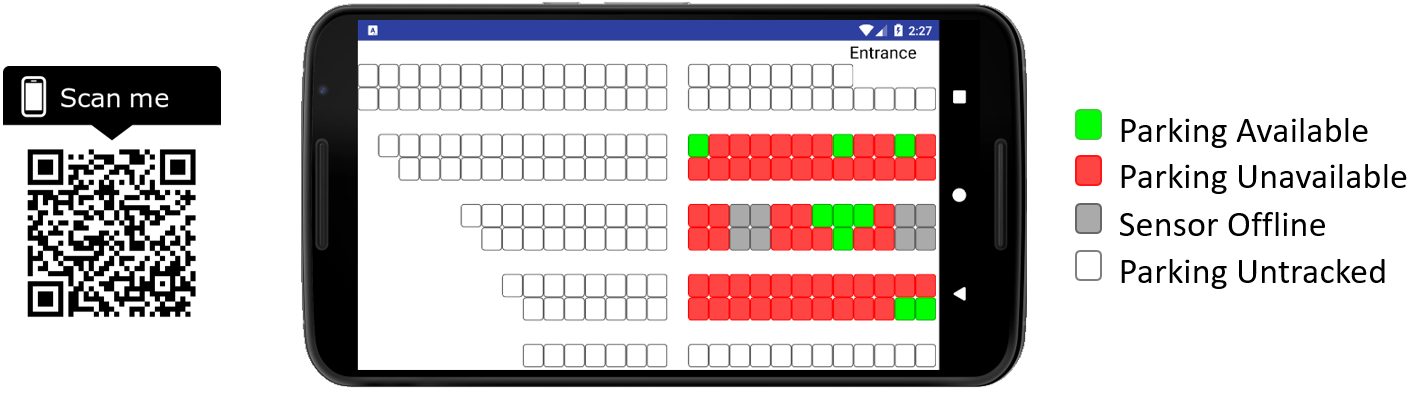
\includegraphics[width=0.9\columnwidth]{app_screenshot3}
			\captionof{figure}{Screenshot of the developed mobile application }
			\raggedright
		\end{center}
	
	\end{multicols}
	
}


\headerbox{Results \& Evaluation}{name=deployandeval,column=3,row=0,span=1}{
	
	\textbf{System performance}
		\begin{itemize}[leftmargin=13pt]\compresslist
			\item Estimated lifetime on a single charge cycle is 276~days, limited by the highest consumption node
			\begin{center}
				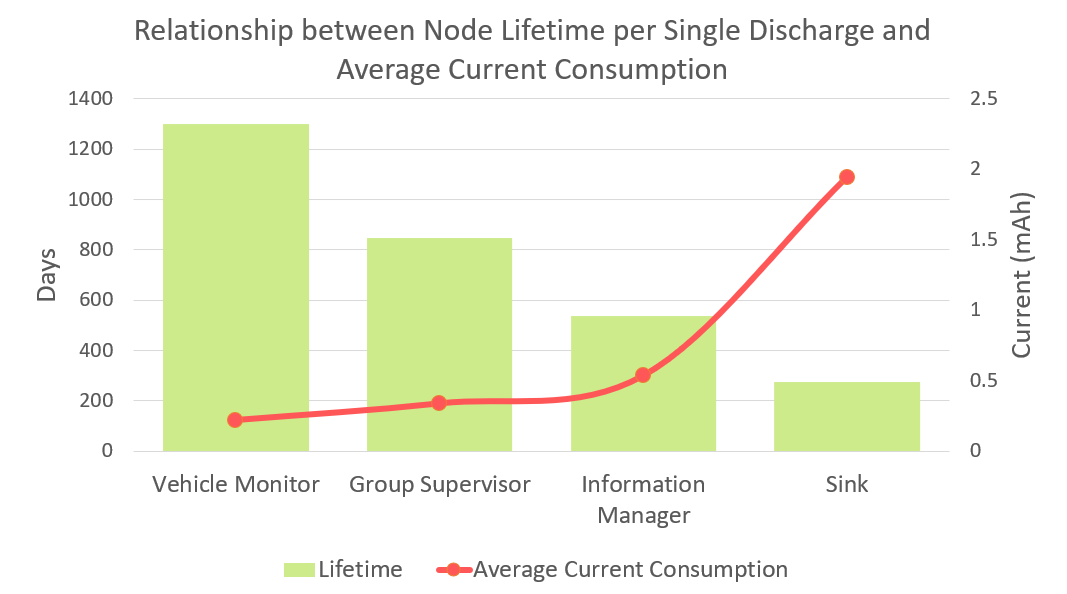
\includegraphics[width=0.8\columnwidth]{consumption}
				\captionof{figure}{Energy performance of the designed system}
			\end{center}
			\item Data consumption of the implemented smart parking system is approximately 3.7~MB per month, and scales non-linearly with parking lot size
			\begin{center}
				\resizebox{0.9\textwidth}{!}{
					\begin{tabular}{c c c}
						\toprule
						\textbf{Number of Parkings} & \textbf{Payload Size (B)} & \textbf{Monthly Usage (MB)}\\
						\midrule
						1 & 60 & 0.08 \\
						72 & 262 & 3.77 \\
						192 & 582 & 8.38 \\
						\bottomrule
					\end{tabular}
				}
			\captionof{table}{Effect of parking lot size on WSN data consumption}
			\end{center}
			\item Mobile application data consumption is minimal with a refresh interval of 5~seconds
			\item Requests for data which has not been updated incur a cost of only 4~kB per request
			\item At the current scale, the calculated price per node is  R~273.52, with a cost-per-parking of R~68.38
		\end{itemize}
	}
	

\headerbox{Future Work}{name=futurework,column=3,row=1,span=1, below=deployandeval}{
		\begin{itemize}[leftmargin=13pt]\compresslist
		\item Sensors take multiple consecutive readings and use this information to distinguish between the type of object being sensed. This will avoid false positives from pedestrians or other objects crossing the sensor path temporarily.
		\item Mobile application updates, including the option to manually refresh the parking lot information.
	\end{itemize}
}

\headerbox{Conclusions}{name=conclusion,column=3,span=1,row=3,below=futurework,above=bottom}{
	\vspace{1.5mm}
	A scalable IoT-based smart parking system has been designed which communicates parking bay availability to drivers via a mobile application. The expected lifetime of the system is 276 days and incurs a monthly data cost of only 3.77~MB. Implementing the system for 72 parking bays results in a cost-per-parking of R~68.38. The ParkSmart system meets all of its objectives, making the project a success.
}

%\headerbox{References}{name=references,column=3,span=1,above=bottom}{
%	
%}

\end{poster}

\end{document}